\documentclass[12pt,reqno]{amsart}
\usepackage[T1]{fontenc}
\usepackage[utf8]{inputenc}
\usepackage{amsmath, amssymb, graphicx, hyperref, comment}
\usepackage{caption, subcaption}
\usepackage{adjustbox}
\usepackage[margin=1in,marginparwidth=0.75in]{geometry}
\usepackage{bm}

\hypersetup{
    colorlinks=true,
    linkcolor=blue,
    filecolor=black,      
    urlcolor=blue,
    citecolor=blue,
}

\newcommand\marginal[1]{\marginpar{\raggedright\parindent=0pt\tiny #1}}

\newtheorem{theorem}{Theorem}[section]
\newtheorem*{theorem*}{Theorem}
\newtheorem{lemma}[theorem]{Lemma}
\newtheorem*{lemma*}{Lemma}
\newtheorem{corollary}[theorem]{Corollary}
\newtheorem*{corollary*}{Corollary}
\newtheorem{prop}[theorem]{Proposition}
\newtheorem*{prop*}{Proposition}
\newtheorem{observation}[theorem]{Observation}
\newtheorem{construction}[theorem]{Construction}


\newtheorem{conjecture}[theorem]{Conjecture}
\newtheorem{question}[theorem]{Question}
\newtheorem{obs}[theorem]{Observation}
\newtheorem{claim}[theorem]{Claim}
\newtheorem{fact}[theorem]{Fact}

\theoremstyle{definition}
\newtheorem{definition}[theorem]{Definition}
\newtheorem*{definition*}{Definition}
\theoremstyle{remark}
\newtheorem{remark}[theorem]{Remark}

% theorems
\usepackage{thmtools}
\usepackage{thm-restate}

\usepackage{lipsum}


\DeclareMathOperator{\dist}{dist}
\DeclareMathOperator{\aut}{Aut}
\DeclareMathOperator{\gal}{Gal}
\DeclareMathOperator{\var}{\textbf{var}}
\DeclareMathOperator{\orb}{Orb}
\DeclareMathOperator{\ff}{Frac}
\DeclareMathOperator{\stab}{Stab}
\DeclareMathOperator{\inn}{Inn}
\DeclareMathOperator{\Ind}{Ind}
\DeclareMathOperator{\Res}{Res}
\DeclareMathOperator{\spn}{Span}
\DeclareMathOperator{\out}{Out}
\DeclareMathOperator{\ima}{Im}
\DeclareMathOperator{\dom}{Dom}
\DeclareMathOperator{\rk}{rk}
\DeclareMathOperator{\disc}{disc}
\DeclareMathOperator{\tors}{Tors}
\DeclareMathOperator{\Mor}{Mor}
\DeclareMathOperator{\End}{End}
\DeclareMathOperator{\Hom}{Hom}
\DeclareMathOperator{\Nat}{Nat}
\DeclareMathOperator{\spec}{Spec}
\DeclareMathOperator{\ann}{Ann}
\DeclareMathOperator{\ord}{ord}
\DeclareMathOperator{\conjc}{Conj}
\DeclareMathOperator{\Br}{Br}
\DeclareMathOperator{\Tr}{Tr}
\DeclareMathOperator{\Nm}{Nm}
\DeclareMathOperator{\Char}{char}
\DeclareMathOperator{\crossing}{cr}
\graphicspath{{Figures/}}

%────────────────────────────────────────────────────────────────────────────────────────────────────────────────────────────────────────────────────
%────────────────────────────────────────────────────────────────────────────────────────────────────────────────────────────────────────────────────

\begin{document}
\title{\textbf{TITLE}} 

%%%% DEPARTMENT OF MATHEMATICS???????? Why not CAS?

\author[Cushman]{Adam Cushman}
\address{Department of Mathematics\\
         Indiana University,
         Bloomington, IN 47405
         USA} 
\email{acushma@iu.edu}
\date{\today}

\begin{abstract}
The sum-product conjecture, posed in 1983 by Erd{\H{o}}s and Szemer{\'e}di \cite{erdos-szemeredi}, 
posits that any sufficiently large set must have a `relatively large' number
of distinct sums or products between its elements.
A newer conjecture extends this idea, positing that for convex sets there must be a `relatively large'
number of distinct sums between its elements. Both conjectures remain open and far from being solved.
This report provides an entirely self-contained overview of some known results and the methods
used to achieve them.
\end{abstract}

\maketitle

%────────────────────────────────────────────────────────────────────────────────────────────────────────────────────────────────────────────────────
%────────────────────────────────────────────────────────────────────────────────────────────────────────────────────────────────────────────────────

\textbf{motivate erdos multiplication table}

\textbf{issue of "for any set A" in statements, but only as A gets sufficiently large}

\textbf{GO THROUGH WHOLE THING AND USE TILDE NOTATION}

\textbf{introduce f(A) notation}

\section{Introduction and Motivation} 

For any sets \(A,B\) and binary operation \(\cdot \) which acts on elements of \(A\) and \(B\), we define
\[
    A \cdot  B = \left\{ a \cdot  b : a \in A~,~ b \in B \right\} 
.\]

Observe the following example which motivates the study of the sum-product problem.

Let \(A = \left\{ 1, 2, 3, \cdots, n \right\}\) and \(G = \left\{ 2, 2^{2}, 2^{3}, \cdots , 2^{n} \right\}\).

Notice that \(A\) is given by an arithmetic sequence and \(G\) by a geometric sequence.
We are going to calculate \(\left\lvert A+A \right\rvert , \left\lvert AA \right\rvert , \left\lvert G+G \right\rvert ,\) and \(\left\lvert GG \right\rvert \).

Observe that
\begin{align*}
    \left\lvert A + A \right\rvert  & = \left\lvert \left\{2,3, \cdots ,2n \right\}  \right\rvert \\
    & = 2n - 1 \\
    & = 2 \left\lvert A \right\rvert - 1,
\end{align*}
and by the same argument,
\begin{align*}
    \left\lvert GG \right\rvert  & = \left\lvert \left\{2^{2}, 2^{3}, \cdots , 2^{2n} \right\} \right\rvert  \\
    & =2 \left\lvert G \right\rvert -1.
\end{align*}
We have
\begin{align*}
    \left\lvert G + G \right\rvert & = \left\lvert \left\{ 2^{i} + 2^{j} : i,j \in \left\{ 1, \cdots , n \right\} \right\} \right\rvert
\end{align*}
For all \(i,j\), \(2^{i} + 2^{j}\) is a number written in base \(2\). By the uniqueness of representations
in different bases (see appendix), we have that \(2^{i} + 2^{j}\) is distinct for every choice of \(\left\{ i,j \right\} \). Therefore,
\begin{align*}
    \left\lvert G + G \right\rvert & \geq  \left\lvert \left\{ \left\{ i,j \right\} : i,j \in \left\{ 1, \cdots , n \right\}  \right\}  \right\rvert \\
    & = \binom{n}{2} + n \\
    & = \binom{\left\lvert G \right\rvert + 1}{2} 
\end{align*}

Finally, I prove in the appendix that there exists \(c \in \mathbb{R} ^{+}\) such that
\[
    \left\lvert AA \right\rvert \geq  \frac{c \left\lvert A \right\rvert ^{2}}{\log \left( \left\lvert A \right\rvert  \right) }
.\]

Observing the trivial bounds \( 2 \left\lvert S \right\rvert - 1 \leq \left\lvert S \cdot S \right\rvert \leq \binom{\left\lvert S \right\rvert }{2} \) for any set \(S\) and any
commutative operation \(\cdot \), it is clear that both \(AA\) and \(G +G\) are, as \(\left\lvert A \right\rvert, \left\lvert G \right\rvert \to \infty  \), almost as large as they can be,
and \(A + A, GG \) are as small as they can be.

This is the phenomenon which motivates this problem.
One questions is: ``does there exist a set for which neither the sum nor the product set is large?''
The sum-product conjecture states that such a set does not exist. 
Another question we study in this report is: ``what
determines if the sum set is large or the product set is large?'' A
conjecture which partially attacks this question states that the sum set is large
when the set itself is convex.

The rest of the report will proceed in the following way : \textbf{finish this}

\section{Preliminaries}

As a useful shorthand, for any natural number \(n\), let
\[
    [n] = \left\{ 1, 2 , \cdots , n \right\} 
.\]

The study of these problems requires the notion of orders of magnitude.
For any functions \(f,g: \mathbb{R}   \to \mathbb{R} \), write
\[
    f(x) \gg g(x) \text{ as } x \to \infty 
\]
if
\[
    \exists x_0,c \in \mathbb{R} ^{+}~~\text{s.t.}~~ x > x_0 \implies \left\lvert f(x) \right\rvert \geq c \left\lvert g(x) \right\rvert  
,\]
write
\[
    f(x) \ll g(x) \text{ as } x \to \infty 
\]
if
\[
     \exists x_0,c \in \mathbb{R} ^{+}~~\text{s.t.}~~ x > x_0 \implies \left\lvert f(x) \right\rvert \leq c \left\lvert g(x) \right\rvert 
,\]
and write
\[
    f(x) \asymp g(x) \text{ as } x \to \infty 
\]
if
\[
    f(x) \ll g(x)  ~ ~ \text{and} ~ ~ f(x) \gg g(x) \text{ as } x \to \infty 
.\]

We write \(\ll _{\epsilon},\gg _{\epsilon} \) if the constant depends on \(\epsilon\). For example,
\[
    f(x) \gg _{\epsilon} g(x) ^{ \epsilon}
\]
means
\[
   \forall \epsilon> 0~,~ f(x) \gg g(x) ^{\epsilon}
.\]
More precisely, there is some function \(c : \mathbb{R} ^{+ }\to \mathbb{R} ^{+}\) so
\[
    \forall \epsilon > 0, \exists x_0\in \mathbb{N} ~~\text{s.t.}~~ x > x_0 \implies \left\lvert f(x) \right\rvert \geq c (\epsilon)\left\lvert g(x) ^{\epsilon} \right\rvert
.\]

We write \(\lesssim , \gtrsim \) if, along with a constant factor, there is also a logarithmic factor.
That is
\[
    f(x) \lesssim  g(x)
\]
if there is some \(c \in \mathbb{R} \) such that
\[
    f(x) \ll \left( \log \left( x \right)  \right) ^{c} g(x)
.\]

Throughout this report, the asymptotic parameter (in this case \(x\)) will always tend to \(\infty \),
so it will no longer be mentioned.
Oftentimes the parameter will not even be in the expression. For example,
if for some set \(A\) we write
\[
    \left\lvert A + A \right\rvert \gg \left\lvert A \right\rvert 
,\]
it is taken to mean that \(A\) is defined implicitly by \(\left\lvert A \right\rvert \), and
\(\left\lvert A \right\rvert \) is the parameter which tends to \(\infty \).

For any sets \(A,B\) and any binary operation \(\cdot \) acting on elements of \(A\) and \(B\), define the representation function
\(r_{A \cdot B} : A \cdot B \to \mathbb{N} \) by
\[
    r_{A \cdot B} (x) = \left\lvert \left\{ (a,b)\in  A \times B : x = a \cdot b \right\}  \right\rvert
.\]

Throughout this report the shorthand
\[
    \delta_{A,B} (x) = r_{A - B} (x)~,~ \sigma _{A,B} (x) = r_{A + B} (x)~,~ \delta_{A} (x) = \delta_{A,A} (x) ~,~ \sigma_{A} (x) = \sigma _{A,A} (x)
\]
will be used.

For any sets \(A,B\), define the Additive Energy \(E(A,B)\) and Multiplicative Energy \(M(A,B)\) by
\[
    E(A,B) = \left\lvert \left\{ (a_1,a_2,b_1,b_2) \in A^{2} \times B^{2} : a_1 - b_1 = a_2 - b_2 \right\}  \right\rvert 
\]
and
\[
    M(A,B) = \left\lvert \left\{ (a_1,a_2,b_1,b_2)\in  A^{2} \times B^{2} : \frac{a_1}{b_1}  = \frac{a_2}{b_2}  \right\}  \right\rvert
.\]

Observe that
\[
    E(A,B) = \sum _{x \in A - B} \delta_{A,B} (x)^{2}
\]
and
\[
    M(A,B) = \sum _{x \in \frac{A}{B} } r_{\frac{A}{B} } (x)^{2} 
.\]

This definition is symmetric in the sense that a 4-tuple \((a_1,a_2,b_1,b_2)\in A^{2} \times B^{2}\) is a solution to
\[
    a_1 - b_1 = a_2 - b_2
\]
if and only if it is a solution to
\[
    a_1+b_2 = a_2+b_1
,\]
and therefore
\[
    E(A,B) =\sum _{x \in A - B} \delta_{A,B}  (x)^{2} = \sum _{x \in A + B} \sigma_{A,B}  (x)^{2}
.\]

There is a similar argument for multiplicative energy.
Any 4-tuple \((a_1,a_2,b_1,b_2) \in A^{2} \times B^{2}\) with nonzero entries is a solution to
\[
    \frac{a_1}{b_1} = \frac{a_2}{b_2}
\]
if and only if it is a solution to
\[
    a_1 b_2 = a_2 b_1
.\]
There are at most
\[
    \sum _{i = 1} ^{4} \binom{4}{i}  = 15
\]
4-tuples with zero entries, so
\[
    M(A,B) = \sum _{x \in \frac{A}{B} } r_{\frac{A}{B} } (x) ^{2} \asymp \sum _{x \in AB} r_{AB} (x)^{2}
.\]

We also define higher energies
\[
    E_{n} (A,B) = \sum _{x \in A-B} \delta_{A,B} (x)^{n}  
,\]
so
\[
    E(A) = E_{2} (A)
,\]
and as a shorthand use
\[
    E_{n} (A) = E_{n} (A,A)
.\]
Similar definitions and shorthand are used for multiplicative energy.

We can relate the energies to the sizes of the sum and product sets by the Cauchy-Schwarz Inequality.
\[
    \left\lvert A \right\rvert \left\lvert B \right\rvert = \sum _{x \in A + B} \sigma_{A,B}  (x) \leq \left\lvert A + B \right\rvert ^{\frac{1}{2} } E(A,B)^{\frac{1}{2} }
,\]
and
\[
    \left\lvert A \right\rvert \left\lvert B \right\rvert = \sum _{x \in AB} r_{AB} (x) \leq \left\lvert AB \right\rvert ^{\frac{1}{2} }M(A,B)^{\frac{1}{2} }
.\]
Similar inequalities can be derived for \(\left\lvert A-B \right\rvert \) and \(\left\lvert \frac{A}{B}  \right\rvert \).

Let \(I \subset \mathbb{R} \) be an interval. 
    We call a function \(f: I \to \mathbb{R} \) convex if for
    any 2 points \(x_1,x_2 \in I\), and any \(\lambda \in [0,1]\),
    \[
        f((x_1-x_2)\lambda + x_2) \leq \left( f(x_1)-f(x_2) \right) \lambda + f(x_2)
    .\]

    A finite set \(A \subset \mathbb{R}\) is convex if there is a function \(f: [1, \left\lvert A \right\rvert ] \to \mathbb{R} \)
such that
\[
    A = \left\{ f(i) : i \in \left\{ 1, \cdots , \left\lvert A \right\rvert  \right\}  \right\} 
.\]

A property of convex functions which will come up later, and is worth proving now, is
\begin{lemma}
Let \(I \subset \mathbb{R} \) be an interval. Let \(f : I \to \mathbb{R} \) be convex. Let \(T \subset \mathbb{R} ^{2}\).

Take \(\ell  = \left\{ (x,f(x)) : x \in I \right\} \) to be the graph of \(f\). We have that
\[
    \forall t_1,t_2 \in T ~,~ \left\lvert \left( \ell + t_1 \right) \cap \left( \ell +  t_2 \right)  \right\rvert   \leq  1
.\]

That is that translations of the graph of a convex function intersect in at most one point.
\end{lemma}

\begin{proof}
\textbf{PROVE THIS}
\end{proof}

\textbf{Dyadic partitioning introduction}

%────────────────────────────────────────────────────────────────────────────────────────────────────────────────────────────────────────────────────
%────────────────────────────────────────────────────────────────────────────────────────────────────────────────────────────────────────────────────


\section{Statement of Problems}

We'll now move on to precise statements of the mentioned problems, and statements of the most modern results.

The idea that there does not exist a set with a small sum and product set is
stated precisely as
\begin{conjecture}[Sum-Product Conjecture]
For every finite set \(A \subset \mathbb{R} \),
\[
    \max \left( \left\lvert A+A \right\rvert, \left\lvert A \cdot A \right\rvert  \right) \gtrsim   \left\lvert A \right\rvert^{2}
\]
\end{conjecture}

The idea that convexity opposes additive structure is stated precisely as

\begin{conjecture}[Convex Sumset Conjecture]
    For finite and convex set \(A\),
    \[
        \left\lvert A+A \right\rvert \gtrsim   \left\lvert A \right\rvert ^{2}
    \]
\end{conjecture}

To date, the best results for both of these conjectures are proven in \cite{stevens-rudnev}.
\begin{theorem}
    For every sufficiently large finite set \(A \subset \mathbb{R} \),
    \[
        \max \left( \left\lvert A+A \right\rvert ~,~ \left\lvert A \cdot A \right\rvert  \right) \gtrsim    \left\lvert A \right\rvert^{\frac{4}{3} + \frac{2}{1167}}
    \]
\end{theorem}
and
\begin{theorem}
    For every sufficiently large, finite, and convex set \(A\),
    \[
        \left\lvert A+A \right\rvert \gtrsim   \left\lvert A \right\rvert ^{\frac{30}{19} }
    \]
\end{theorem}

These results will not be covered in this report. In this report,
the strongest results proven are
\begin{theorem}\label{thm:solymosi-sp}
For finite sets \(A \subset \mathbb{R} \),
\[
    \max \left( \left\lvert A+A \right\rvert , \left\lvert AA \right\rvert  \right) \gtrsim \left\lvert A \right\rvert ^{\frac{4}{3} }
.\]
\end{theorem}
\begin{theorem}\label{thm:shkredov-sum}
For finite and convex sets \(A \subset \mathbb{R} \),
\[
    \left\lvert A + A \right\rvert \gtrsim  \left\lvert A \right\rvert ^{\frac{14}{9} }
.\]
\end{theorem}
and
\begin{theorem}\label{thm:shkredov-diff}
For finite and convex sets \(A \subset \mathbb{R} \),
\[
    \left\lvert A - A \right\rvert \gtrsim \left\lvert A \right\rvert ^{\frac{8}{5} }
.\]
\end{theorem}

Theorem \ref{thm:solymosi-sp} is the weakest amongst these results, although it is
still near the best known result.
Theorem \ref{thm:shkredov-diff} gives the best known exponent on \(\left\lvert A \right\rvert \), and
Theorem \ref{thm:shkredov-sum} is obtained by a slight variation on the same methods.

\section{Graphs and the Crossing Number Inequality}

\textbf{simple, connected}

\textbf{cite szekely and tao}

\textbf{Tao's article reread to see what I missed}

\textbf{First proven in ...}

\textbf{Theres something going on with connectedness here}

%────────────────────────────────────────────────────────────────────────────────────────────────────────────────────────────────────────────────────
%────────────────────────────────────────────────────────────────────────────────────────────────────────────────────────────────────────────────────

\textbf{rewrite this paragraph}

A profoundly useful theorem in the study of sum-product conjectures is the
Szemeredi-Trotter theorem, a statement about systems of points and lines.

The easiest way to prove this theorem is through the use of the crossing number inequality,
a statement about how planar a given graph can be. The purpose of this section is to give a proof
of the crossing number inequality.

Due to the brevity of this report, the definitions and proofs given will not be
as rigorous as they should be. There are also pictures to help understand.

%────────────────────────────────────────────────────────────────────────────────────────────────────────────────────────────────────────────────────
%────────────────────────────────────────────────────────────────────────────────────────────────────────────────────────────────────────────────────


\textbf{define connected}

A graph \(G\) is a pair \(G = (V,E)\) where each \(e \in E\) is of the form \(e \subset V\) with \(\left\lvert e \right\rvert = 2\).
We call the set \(V\) the vertices, and the set \(E\) the edges. A drawing is
a representation of a graph with vertices as points in the plane and edges as curves between their
respective vertices. For example:

\begin{figure}[h]
    \centering
    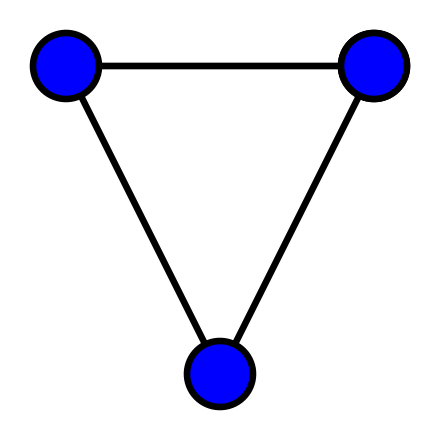
\includegraphics[width=0.1\textwidth]{3graph.png}
    \caption{A drawing of a graph with \(V = \left\{ A,B,C \right\}\) and \(E = \left\{ \left\{ A,B \right\} , \left\{ B,C \right\} ,\left\{ A,C \right\}  \right\} \)}
\end{figure}

A graph is connected if for any 2 vertices, there exists a sequence of edges which join them.
Note that connectedness is a property of a graph and not of the drawing of a graph.

There are infinitely many ways to draw any given graph. A crossing in a drawing
of a graph is an intersection between 2 curves which represent edges. The 
crossing number of a graph is the minimum number of crossings a drawing
of the graph can have. Denote this by
\(\crossing(G)\). A graph \(G\) is called planar if its crossing number is 0.

A precise statement of the Crossing Number Inequality is

\begin{theorem}\label{thm:crossing-number-inequality}
    Let \(G = (V,E)\) be a connected graph. If \(\left\lvert E \right\rvert \geq 4 \left\lvert V \right\rvert \)
    then
    \[
        \crossing\left( G \right) \gg \frac{\left\lvert E \right\rvert ^{3} }{\left\lvert V \right\rvert ^{2}}  
    .\]
\end{theorem}

For a drawing of a planar graph, we call any region of the plane which is bounded by edges a face. We also call
the unbounded region of the plane a face. Here is an example of a drawing of a planar
graph with labelled faces:

\begin{figure}[h]
    \centering
    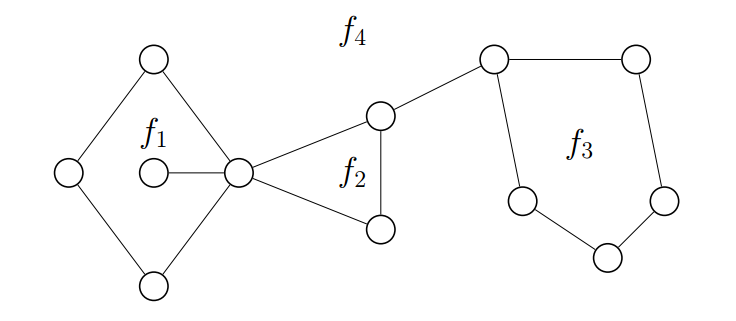
\includegraphics[width=0.4\textwidth]{faceimage.png}
    \caption{Drawing of Planar Graph with Labeled Faces \(f_{i} \)}
\end{figure}

\textbf{cite tao }

Observe that any non-planar graph \(G = (V,E)\) can be turned into a planar graph by removing at most
\(\crossing\left( G \right) \) edges from \(E\). Therefore, a bound on the number of
edges a graph can have and remain planar yields a bound on the crossing number for any graph.
A famous theorem relating the vertices and edges of planar graphs is

\begin{theorem}[Euler's Formula for Planar Graphs]\label{thm:euler-formula-graphs}
Let \(G = (V,E)\) be a connected planar graph, with \(\left\lvert V \right\rvert \geq 1\), and consider some drawing with 0 crossings.
Let \(F\) be the set of all faces of this drawing.
\[
    \left\lvert V \right\rvert - \left\lvert E \right\rvert + \left\lvert F \right\rvert = 2
.\]
\end{theorem}

\begin{proof}
We may construct our drawing of \(G\) by first drawing a vertex, and then doing combination of the following steps: 

\textbf{PROOF}
\end{proof}

The dependence on \(\left\lvert F \right\rvert \) in Euler's formula can be removed by using
its obvious dependence on \(\left\lvert E \right\rvert \). 

We call an edge incident to a face if the edge is one of the bounding edges which define the face. 
Define \(\chi : F \times E \to \left\{ 0,1 \right\} \) as the incidence function, so
\(\chi(f,e) = 1\) if \(f\) and \(e\) are incident, and \(\chi(f,e) = 0\) otherwise.
The total number of face edge incidences is
\[
    I(F,E) = \sum_{f\in F} \sum _{e \in E} \chi(f,e)
.\]

\textbf{JUSTIFY THIS ASSUMPTION SOMEWHERE}
We assume \(\left\lvert E \right\rvert  \geq 3\), so that every face is incident to at least 3 edges.
It follows that
\[
    I \geq \sum _{f \in F} 3 = 3 \left\lvert F \right\rvert 
.\]
Every edge is incident to at most 2 faces, so it follows that
\[
    I \leq \sum _{e \in E} 2 = 2 \left\lvert E \right\rvert 
.\]
Therefore
\[
    3 \left\lvert F \right\rvert \leq 2 \left\lvert E \right\rvert 
\]
or
\[
    \left\lvert F \right\rvert \leq \frac{2}{3} \left\lvert E \right\rvert 
.\]
Applying this to Euler's formula,
\[
    \left\lvert V \right\rvert - \left\lvert E \right\rvert + \frac{2}{3} \left\lvert E \right\rvert \geq 2
\]
or
\[
    \left\lvert E \right\rvert \leq 3 \left\lvert V \right\rvert -6
\]
when \(\left\lvert E \right\rvert \geq 3\).
Now suppose that \(G = (V,E)\) is non-planar and connected. As mentioned before, \(G\) may be turned planar by removing
at most \(\crossing\left( G \right) \) edges.

\textbf{READ TAO AND JUSTIFY ABOVE BETTER}
Therefore, for any graph \(G\) with \(\left\lvert E \right\rvert  \geq 3\),
\[
    \left\lvert E \right\rvert - \crossing\left( G \right) \leq 3 \left\lvert V \right\rvert - 6
\]
or
\[
    \crossing\left( G \right) > \left\lvert E \right\rvert - 3 \left\lvert V \right\rvert 
.\]

To further improve this inequality, we apply the probabilistic method
to the deletion of vertices of \(G\).

Let each \(v \in V\) be
removed with a probability \(1-p~,~  p \in (0,1)\). Let the remaining set of vertices be \(V'\). 

An edge is
removed whenever either of the corresponding vertices are removed. Let the remaining set of edges be \(E'\). Let the remaining graph be
\(G' = (V',E')\). We have that if \(\left\lvert E' \right\rvert \geq 3\),
\[
    \crossing\left( G' \right) \geq \left\lvert E' \right\rvert - 3 \left\lvert V' \right\rvert 
,\]
and so
\[
    \mathbb{E} \left( \crossing\left( G' \right)  \right) \geq \mathbb{E} \left( \left\lvert E' \right\rvert - 3 \left\lvert V' \right\rvert  \right) 
,\]
or, by the linearity of the expected value,
\[
    \mathbb{E} \left( \crossing\left( G' \right)  \right) \geq \mathbb{E} \left( \left\lvert E' \right\rvert  \right) - 3 \mathbb{E} \left( \left\lvert V' \right\rvert  \right)    
.\]
Each \(v \in V\) is removed with probability \(1-p\), so
\[
    \mathbb{E} \left( \left\lvert V' \right\rvert  \right) = p \left\lvert V \right\rvert 
.\]
Each edge remains only when both corresponding vertices remain. Each vertex remains
independently with a probability \(p\), so 
\[
    \mathbb{E} \left( \left\lvert E' \right\rvert  \right) = p^{2}\left\lvert E \right\rvert 
.\]

We can bound \(\mathbb{E} \left( \crossing\left( G' \right)  \right) \) by considering a drawing of \(G\) with the minimum number of crossings. 
Each crossing remains and only when both corresponding edges remain, each of which occurs independently with probability
\(p^{2}\).

The expected value of the number of crossings remaining in the drawing is \(p^{4} \crossing\left( G \right) \).
There is no guarantee that this drawing is optimal to minimize the crossings of \(G'\), but we may conclude that
\[
    \mathbb{E} \left( \crossing\left( G' \right)  \right) \leq p ^{4} \crossing\left( G \right)
,\]
and therefore that
\[
    p^{4} \crossing\left( G \right) \geq \mathbb{E} \left( \crossing\left( G \right)  \right) \geq p^{2} \left\lvert E \right\rvert - 3 p \left\lvert V \right\rvert 
\]
for any \(p \in (0,1)\). 


Because we are only concerned with an order of magnitude bound, we assume \(\left\lvert E \right\rvert \geq 4\left\lvert V \right\rvert \), and take \(p = \frac{4\left\lvert V \right\rvert }{\left\lvert E \right\rvert }\).
This yields the result
\[
    \crossing\left( G \right) \geq \frac{\left\lvert E \right\rvert }{\left( \frac{4 \left\lvert V \right\rvert }{\left\lvert E \right\rvert }   \right)^{2} } - \frac{3 \left\lvert V \right\rvert }{\left( \frac{4 \left\lvert V \right\rvert }{\left\lvert E \right\rvert }  \right) ^{3} } = \frac{1}{16} \left( \frac{\left\lvert E \right\rvert ^{3} }{\left\lvert V \right\rvert ^{2}} - \frac{3 \left\lvert E \right\rvert ^{3} }{4 \left\lvert V \right\rvert ^{2}}  \right) \gg \frac{\left\lvert E \right\rvert ^{3} }{\left\lvert V \right\rvert ^{2}}
.\]

\section{The Szemeredi-Trotter Theorem}

\textbf{LOOK OVER WHOLE SECTION}

\textbf{CONCAVE OR CONVEX}

With this, we can employ the argument of \cite{szekely-SzT} to prove the Szemeredi-Trotter Theorem.
A precise statement of the Szemeredi-Trotter Theorem, first proven in \cite{SzT-original} is

\begin{theorem}[Szemeredi-Trotter Theorem]
Let \(P \subset \mathbb{R} ^{2}\) be a finite set of points. Let \(\mathcal{L} \) be a finite set of curves in \(\mathbb{R} ^{2}\). 

Let \(\chi : P \times \mathcal{L}  \to \left\{ 0,1 \right\} \) be the incidence function
between a point and a line, so
\[
\chi(p,l) = 
\begin{cases}
1 ~ ~ \text{if} ~ ~ p\in l\\
0 ~ ~ \text{otherwise} 
\end{cases}
\]

If any two \( l \in \mathcal{L} \) intersect in at most one point,
then the total number of point-curve incidences,
\[
    I(P, \mathcal{L} ) = \sum _{(p,l)\in P \times \mathcal{L} } \chi(p,l)
\]
satisfies
\[
    I(P,\mathcal{L} ) \ll  \left\lvert P \right\rvert^{\frac{2}{3} } \left\lvert \mathcal{L}  \right\rvert ^{\frac{2}{3} } + \left\lvert P \right\rvert + \left\lvert \mathcal{L}  \right\rvert 
.\]
\end{theorem}

\begin{proof}
This is proven by turning a system of curves and points into a graph. We first omit all points and curves which
contribute to one or fewer incidences. 

For each remaining curve, if there are \(n\) incidences
along it, we partition it into \(n-1\) curves, each with 2 incidences. These become
the edges of the drawing of some graph. Let the set of edges be \(E\).

If \(I_0(P , \mathcal{L} )\) is the remaining number of incidences,
\[
    \left\lvert E \right\rvert \geq  I_0(P , \mathcal{L} ) - \left\lvert \mathcal{L}  \right\rvert 
.\]

Let the vertices of the graph, \(V\), be the remaining points in the system. Obviously, \(\left\lvert V \right\rvert \leq \left\lvert P \right\rvert \).

Because any two curves intersect in at most one point, \(\crossing\left( G \right) \) is at most
\(\left\lvert \mathcal{L}  \right\rvert ^{2}\).

Supposing that \(\left\lvert E \right\rvert \geq 4 \left\lvert V \right\rvert \), we have that
\[
    \left\lvert \mathcal{L}  \right\rvert ^{2} \geq \crossing\left( G \right) \gg \frac{\left( I_0 \left( P, \mathcal{L}  \right) - \left\lvert \mathcal{L}  \right\rvert \right)  ^{3}  }{\left\lvert P \right\rvert ^{2}} 
\]
or
\[
    I_0(P , \mathcal{L} ) \ll \left\lvert \mathcal{L}  \right\rvert ^{\frac{2}{3} } \left\lvert P \right\rvert ^{\frac{2}{3} } + \left\lvert \mathcal{L}  \right\rvert 
.\]

If \(\left\lvert V \right\rvert \geq \frac{1}{4} \left\lvert E \right\rvert \), then \(\left\lvert V \right\rvert  \gg \left\lvert E \right\rvert \), or
\[
    \left\lvert P \right\rvert \gg I_0\left( P , \mathcal{L}  \right) - \left\lvert \mathcal{L}  \right\rvert \implies I_0(P,\mathcal{L} ) \ll \left\lvert P \right\rvert  + \left\lvert \mathcal{L}  \right\rvert  
.\]

Finally, the remaining incidences not yet counted is 
\[
    I(P, \mathcal{L} ) - I_0 (P , \mathcal{L} ) \ll \left\lvert \mathcal{L} \right\rvert + \left\lvert P \right\rvert
,\]
so
\[
    I(P, \mathcal{L} ) \ll \left\lvert P \right\rvert ^{\frac{2}{3} }\left\lvert \mathcal{L}  \right\rvert ^{\frac{2}{3} } + \left\lvert P \right\rvert + \left\lvert \mathcal{L}  \right\rvert 
.\]
\end{proof}

The Szemeredi Trotter theorem has a handful of direct applications to the sum
product conjecture and the convex sumset conjecture. The main theorem which leads
to these results is proven in \cite{elekes}.

\begin{theorem} \label{thm:translations-of-convex-szt}
Let \(A \subset \mathbb{R} \) be finite, with \(\left\lvert A \right\rvert = n\). 

Label the
elements of \(A\) so that \(a_1 < a_2 < \cdots < a_{n} \). 

Let \(f : [a_1,a_{n} ] \to \mathbb{R} \) be convex. Let \(S = \left\{ (a,f(a)) : a \in A \right\} \) and \(T \subset \mathbb{R} ^{2}\) be finite. 

We have
\[
    \left\lvert S + T \right\rvert \gg \max \left( \left\lvert S \right\rvert ^{\frac{3}{2} } \left\lvert T \right\rvert ^{\frac{1}{2} } , \left\lvert S \right\rvert \left\lvert T \right\rvert  \right)
.\]
\end{theorem}

\begin{proof}
    Let
    \[
        L_{t} = \left\{ (x,f(x)) + t : x \in [a_1,a_{n} ], t \in T \right\} 
    ,\]
    and let
    \[
        \mathcal{L} = \left\{ L_{t} : t \in T \right\} 
    .\]
    For every \(x \in A\), \((x,f(x)) + t \in S + T\). Therefore, there are \(\left\lvert A \right\rvert = \left\lvert S \right\rvert \) incidences
    between \(L_{t} \) and the point set \(S + T\), for all \(t \in T\). It follows that there are \(\left\lvert S \right\rvert \left\lvert T \right\rvert \)
    total incidences. The set \(\mathcal{L} \) consists of
    translations of the graph of a convex function, so the Szemeredi-Trotter theorem is satisfied. Thus
    
    \[
        \left\lvert S \right\rvert \left\lvert T \right\rvert \ll \left\lvert S + T \right\rvert ^{\frac{2}{3} } \left\lvert T \right\rvert ^{\frac{2}{3} } + \left\lvert S + T \right\rvert + \left\lvert T \right\rvert 
    .\]
    Trivially,
    \[
        \left\lvert S + T \right\rvert \geq \left\lvert T \right\rvert 
    ,\]
    so
    \[
        \left\lvert S \right\rvert \left\lvert T \right\rvert  \ll\max \left( \left\lvert S + T \right\rvert ^{\frac{2}{3} }\left\lvert T \right\rvert ^{\frac{2}{3} }, \left\lvert S+T \right\rvert  \right) 
    ,\]
    or
    \[
        \left\lvert S + T \right\rvert \gg \max \left( \left\lvert S \right\rvert ^{\frac{3}{2} } \left\lvert T \right\rvert ^{\frac{1}{2} }, \left\lvert S \right\rvert \left\lvert T \right\rvert  \right) 
    .\]
\end{proof}

The following corollaries are also proven in \cite{elekes}.

\begin{corollary}
    For convex and finite sets \(A \subset \mathbb{R} \), and finite sets \(B \subset \mathbb{R} \),
    \[
        \left\lvert A + B \right\rvert \gg \left\lvert A \right\rvert \left\lvert B \right\rvert ^{\frac{1}{2} }
    .\]
\end{corollary}
    
\begin{proof}
Let \(A \subset \mathbb{R} \) be finite. Let \(n = \left\lvert A \right\rvert \). Let \(f : [1,n] \to \mathbb{R} \) be the
convex function for which
\[
    A = \left\{ f(i) : i \in [n] \right\} 
.\]
Take
\[
    S = \left\{ (i,f(i)) : i \in [n]\right\} 
\]
and
\[
    T = [n] \times B
.\]
We have
\[
    S + T \subset \left( [n] + [n] \right)  \times \left( A + B \right) 
,\]
so
\[
    \left\lvert S + T \right\rvert \leq \left\lvert [n] + [n] \right\rvert \left\lvert A + B \right\rvert \ll \left\lvert A \right\rvert \left\lvert A + B \right\rvert 
.\]
Apply Theorem \ref{thm:translations-of-convex-szt} to get
\[
    \left\lvert A \right\rvert \left\lvert A + B \right\rvert \gg \left\lvert S + T \right\rvert \gg \max \left( \left\lvert A \right\rvert ^{\frac{3}{2} }\left( \left\lvert A \right\rvert \left\lvert B \right\rvert  \right) ^{\frac{1}{2} }, \left\lvert A \right\rvert \left( \left\lvert A \right\rvert \left\lvert B \right\rvert  \right)  \right) 
\]
or
\[
    \left\lvert A \right\rvert \left\lvert A + B \right\rvert \gg \left\lvert A \right\rvert ^{2}\left\lvert B \right\rvert ^{\frac{1}{2} } \implies  \left\lvert A + B \right\rvert \gg \left\lvert A \right\rvert \left\lvert B \right\rvert ^{\frac{1}{2} }
.\]
\end{proof}

This will be used to achieve stronger results later, but in particular, this gives the result
\begin{corollary}
For sufficiently large sets \(A \subset \mathbb{R} \) which are finite and convex,
\[
    \left\lvert A+A \right\rvert \gg \left\lvert A \right\rvert ^{\frac{3}{2} }
.\]
\end{corollary}

We can also use Theorem \ref{thm:translations-of-convex-szt} to get a result
on the Sum-Product conjecture.
\begin{corollary}
    For finite sets \(A \subset \mathbb{R}^{+} \) of positive real numbers,
    \[
        \max \left( \left\lvert A+A \right\rvert, \left\lvert A\cdot A \right\rvert  \right) \gg \left\lvert A \right\rvert ^{\frac{5}{4} }
    .\]
\end{corollary}

\begin{proof}
Let \(A \subset \mathbb{R} \) be finite. 

Label the elements of \(A\) so that \(a_1 < \cdots < a_{n} \).
Let \(f : [a_1,a_{n} ] \to \mathbb{R} \) be concave or convex.
Take
\[
    S = \left\{ (a,f(a)) : a \in A \right\} 
,\]
and
\[
    T = A \times f(A)
.\]
Observe that
\[
    S + T \subset \left( A + A \right) \times \left( f(A) + f(A) \right) 
,\]
so that
\[
    \left\lvert S + T \right\rvert \ll \left\lvert A + A \right\rvert \left\lvert f(A) + f(A) \right\rvert
.\]

Apply Theorem \ref{thm:translations-of-convex-szt} to get
\[
    \left\lvert A+A \right\rvert \left\lvert f(A) + f(A) \right\rvert \gg \left\lvert S+T \right\rvert \gg \max \left( \left\lvert A \right\rvert ^{\frac{3}{2} } \left( \left\lvert A \right\rvert ^{2} \right) ^{\frac{1}{2} }, \left\lvert A \right\rvert \left\lvert A \right\rvert ^{2} \right) 
\]
or
\[
    \max \left( \left\lvert A + A \right\rvert , \left\lvert f(A) + f(A) \right\rvert  \right) \gg \left\lvert A \right\rvert ^{\frac{5}{4} }
\]
for any convex or concave function \(f : [a_1,a_{n} ] \to \mathbb{R}\).

If \(A \subset \mathbb{R} ^{+}\), we may take \(f(x) = \log \left( x \right) \), immediately yielding the desired result.
\end{proof}

The Szemeredi-Trotter theorem also provides more general tools which can be
used alongside other results to sharpen the above bounds.

\begin{theorem}

    Let \(A \subset \mathbb{R} \) be convex, then for every 
    finite set \(B \subset \mathbb{R} \) we have

    \[
        \left\lvert \left\{ x \in A-B : \delta_{A,B} (x) \geq \tau \right\}  \right\rvert \ll \frac{\left\lvert A \right\rvert \left\lvert B \right\rvert^{2} }{\tau^{3} }
    .\]
\end{theorem}

\begin{proof}
\textbf{PROOF}
\end{proof}

An immediate corollary of this is

\begin{corollary}
Let \(A \subset \mathbb{R} \) be a convex and finite set. Let \(B \subset \mathbb{R} \) be finite.
Order elements \(s_{i} \in A-B\) such that 
\[
    \delta_{A,B} (s_1) \geq \delta_{A,B} (s_2) \geq \cdots \geq \delta_{A,B} (s _{\left\lvert A - B \right\rvert } )
.\]
For every \(1 \leq r \leq \left\lvert A - B \right\rvert\) we have
\[
    \delta_{A,B} (s _{r} ) \ll \frac{\left\lvert A \right\rvert^{\frac{1}{3} } \left\lvert B \right\rvert ^{\frac{2}{3} } }{r^{\frac{1}{3} }}
.\]
\end{corollary}

\begin{proof}
\[
    r = \left\lvert \left\{ x \in A-B : \delta _{A,B} (x) \geq \delta_{A,B} (s _{r} ) \right\}  \right\rvert \ll \frac{\left\lvert A \right\rvert \left\lvert B \right\rvert ^{2} }{\delta_{A,B} (s _{r} )^{3} } \implies \delta_{A} (s _{r} ) \ll \frac{\left\lvert A \right\rvert ^{\frac{1}{3} } \left\lvert B \right\rvert ^{\frac{2}{3} }}{r^{\frac{1}{3} }}
.\]
\end{proof}

Later in the next section we'll use these results to find bounds on the additive
energies between certain sets, but first we'll introduce some simpler results which
use additive and multiplicative energy to show why such bounds are useful.

\section{Additive and Multiplicative Energy Estimates}

Recall that
\[
    \left\lvert A + A \right\rvert \geq  \frac{\left\lvert A \right\rvert ^{4}}{ E(A) }
\]
and
\[
    \left\lvert AA \right\rvert \geq \frac{\left\lvert A \right\rvert ^{4}}{M(A) }
.\]

Observe that finding an upper bound on \(E(A)\) or \(M(A)\) in terms of \(\left\lvert A + A \right\rvert, \left\lvert AA \right\rvert    \), and \(\left\lvert A \right\rvert \)
yields a sum product theorem. In this section we showcase a result which employs this idea.
We also give other, more complicated, estimates on additive energies involving a convex set which
will be used later.

The aforementioned result is Theorem \ref{thm:solymosi-sp}, found in \cite{Solymosi}. It gives a stronger result
on the sum-product conjecture than the Szemeredi-Trotter theorem. 

\textbf{THIS IS A RECALL THEOREM}
\begin{theorem}\label{thm:solymosi}
Let \(A \subset \mathbb{R}^{+} \) be finite.
\[
    \max \left( \left\lvert A+A \right\rvert , \left\lvert AA \right\rvert  \right) \gtrsim  \left\lvert A \right\rvert ^{\frac{4}{3}}
.\]
\end{theorem}

\begin{proof}

We begin with a construction. Consider the set \(A^{2}\), along with the smallest set of lines
through the origin which cover \(A^{2}\).

\begin{figure}[h]
    \centering
    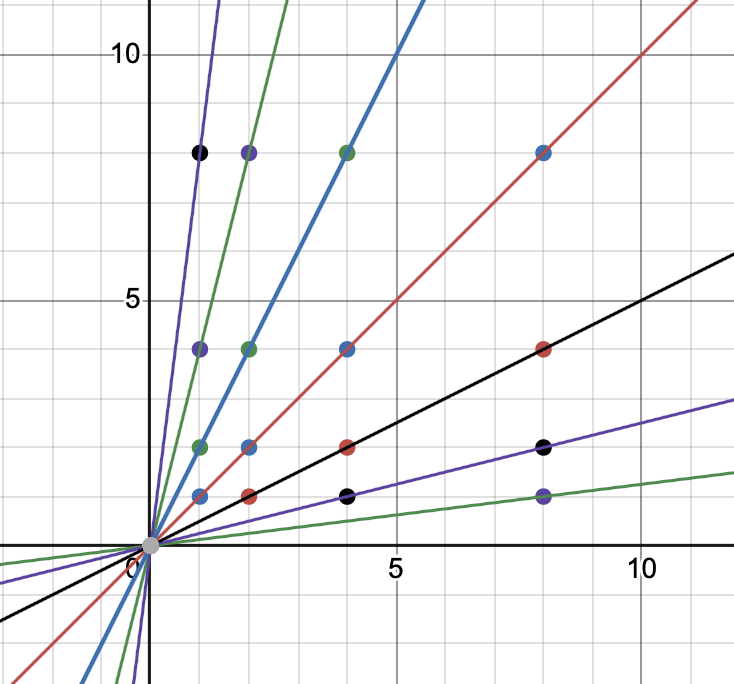
\includegraphics[width=0.5\textwidth]{Sol1.png}
    \caption{Example with \(A = \left\{ 1,2,4,8 \right\} \).}
\end{figure}

The claim is that each line represents an element of \(\frac{A}{A} \). This is
easy to see, two pairs \((a_1,a_2),(b_1,b_2) \in A^{2}\) give the same representation as a quotient if
and only if
\[
    \frac{a_2}{a_1} = \frac{b_2}{b_1} 
.\]
Observe that this is the slope of the line through the origin and the points \((a_1,a_2), (b_1,b_2)\).
This shows that the number of lines in the construction is \(\left\lvert \frac{A}{A}  \right\rvert \), the slope
of each line is an element in \(\frac{A}{A} \), and the number of points on a line
of slope \(m\) is the number of representations of \(m\) as a quotient, \(r_{\frac{A}{A} } (m)\).

We'll now prove 2 facts about the set of vector sums of 2 points lying on consecutive lines.

\begin{figure}[h]
    \centering
    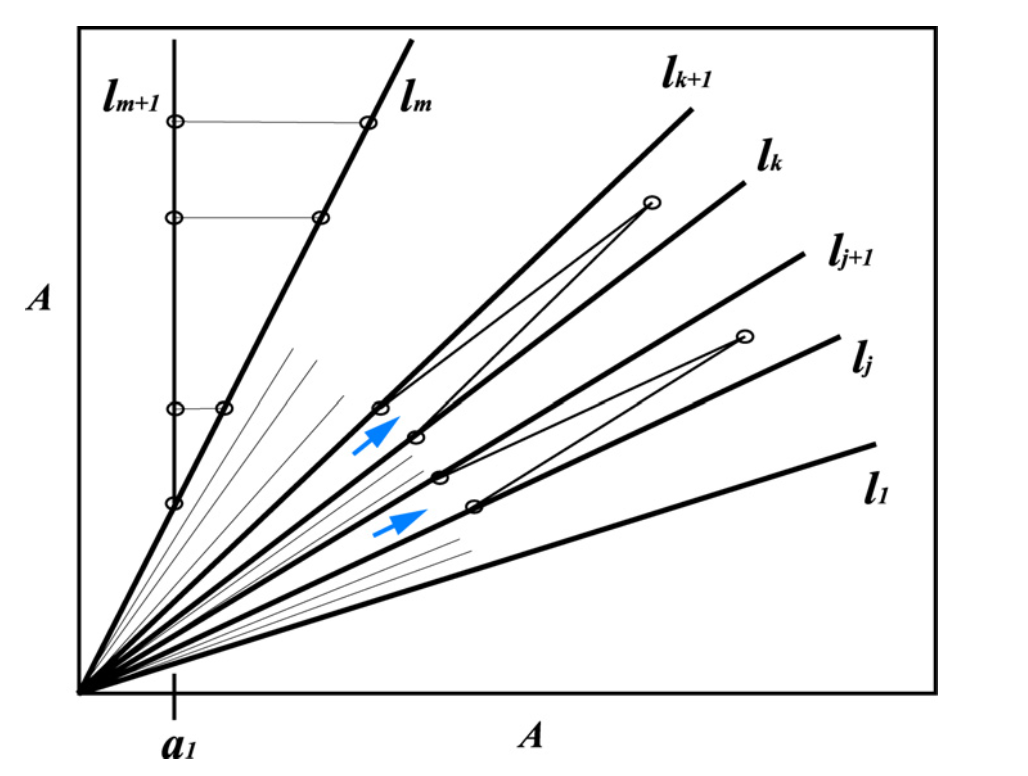
\includegraphics[width=0.5\textwidth]{sol2.png}
    \caption{Vector sums of 2 points lying on consecutive lines. Figure taken from \cite{Solymosi}, where the argument was first given.}
    \label{fig:solymosi}
\end{figure}

Firstly, that the set of vector sums of points along either line is disjoint for each
choice of consecutive lines. In figure \ref{fig:solymosi}, this is represented by the blue arrow between lines
\(l _{j} , l _{j + 1} \) and \(l _{k}  , l _{k+1} \).
To show this, consider 2 consecutive lines and the set of all vector sums between a point on each line.
If our points are \(\left( a_1,a_2 \right)\) and \(\left( b_1,b_2 \right) \), with
\[
    \frac{a_2}{a_1} > \frac{b_2}{b_1}
,\]
then the slope of their sum is
\[
    \frac{a_2+b_2}{a_1+b_1}
\]
which satisfies
\[
    \frac{b_2}{b_1} < \frac{a_2+b_2}{a_1+b_1} < \frac{a_2}{a_1}
.\]
That is, the vector sum must ``lie between'' the two lines which the original vectors are on.
A consequence of this is that, for any pairs of consecutive lines, 
the vector sums of all points along the lines are disjoint.

The remaining claim is that for any choice of points on consecutive lines, the vector sum is distinct.
To show this, consider solutions to
\[
    \lambda_1 v + \lambda_2 w = \lambda_3 v + \lambda_4 w
.\]
We have a solution if and only if
\[
    \left( \lambda_1 - \lambda_3 \right) v + \left( \lambda_2 - \lambda_4 \right) w = 0 
,\]
where \(\lambda_1 \neq \lambda_3\) or \(\lambda_2 \neq \lambda_4\).
This exists only if \(v\) and \(w\) are linearly dependent, which is untrue if
\(\spn{ \left( v \right) } , \spn{ \left( w \right) } \) are distinct lines in \(\mathbb{R} ^{2}\).

We are able to use these facts to prove Theorem \ref{thm:solymosi-sp}.
Begin by applying dyadic partitioning on \(M(A)\) to get
\[
    M(A) = \sum _{x \in \frac{A}{A} } r_{\frac{A}{A} } (x)^{2} \ll  \log \left( \left\lvert \frac{A}{A} \right\rvert   \right) \tau ^{2} \left\lvert S \right\rvert
\]
for some \(\tau\), where \(S = \left\{ x \in \frac{A}{A}  : r_{\frac{A}{A} } (x) \asymp \tau \right\} \).

Consider a reduced system of points and lines, consisting only of the \(\left\lvert S \right\rvert \) many lines which
have \(\asymp \tau\) many points on them. Consider the set of all vector sums between points over
all consecutive lines. Because all pairs of lines give disjoint sets of sums, each with \(\asymp \tau ^{2}\) many distinct sums, there are
\(\tau^{2}\left\lvert S \right\rvert \) many vector sums. The set of all vector sums between points of \(A^{2}\) is a subset of \((A+A)^{2}\),
so
\[
    \tau^{2} \left\lvert S \right\rvert \leq \left\lvert A+A \right\rvert  ^{2}
.\]
Therefore
\[
    \frac{\left\lvert A \right\rvert ^{4}}{\left\lvert AA\right\rvert } \leq M(A) \ll \log \left( \left\lvert \frac{A}{A} \right\rvert   \right) \left\lvert A + A \right\rvert ^{2} \ll \log \left( \left\lvert A \right\rvert  \right)  \left\lvert A+A \right\rvert  ^{2}
\]
so
\[
    \max \left( \left\lvert A + A \right\rvert , \left\lvert AA \right\rvert  \right) \gtrsim \left\lvert A \right\rvert ^{\frac{4}{3} }
.\]

\end{proof}

\textbf{REWRITE BELOW}
Many arguments involving additive energy estimates are not as straightforward
as finding an upper bound. We are often interested in quantites such as 
\(E(A,A + A), E(A - A), E_{3} (A)\) etc.

In the remaining part of this section, we'll prove theorems concerning these quantities
which we will apply to prove more advanced results in the next section. Both of these
results come as corollaries of the Szemeredi-Trotter Theorem.

\begin{theorem}
For convex sets \(A \subset \mathbb{R} \) which are finite and sufficiently large,
\[
    E_{3} (A) \lesssim  \left\lvert A \right\rvert ^{ 3}
.\]
\end{theorem}

\begin{proof}
Recall that upon ordering \(a_{i} \) such that \(\delta_A(a_1) \geq \delta_A(a_2) \geq \dots \geq \delta_{A} (a_{\left\lvert A-A \right\rvert } )\),
we have that
\[
    \delta_{A} (a_{r} ) \ll \frac{\left\lvert A \right\rvert }{r^{\frac{1}{3} }}
.\]

With this,
\begin{align*}
E_3(A) & = \sum _{x \in A-A} \delta_{A} (x)^{3} \\
& \ll \left\lvert A \right\rvert ^{3} \sum_{r=1}^{\left\lvert A-A \right\rvert } \frac{1}{r}\\
& \asymp \left\lvert A \right\rvert ^{3} \int_{1}^{\left\lvert A-A \right\rvert } \frac{1}{r}  ~\mathrm{d} r \\
& \asymp  \left\lvert A \right\rvert ^{3} \log \left( \left\lvert A-A \right\rvert  \right) \\
& \lesssim  \left\lvert A \right\rvert ^{3}
\end{align*}
\end{proof}

\begin{theorem} \label{thm:szt-energy-convex-and-arbitrary}
For convex sets \(A \subset \mathbb{R} \) which are finite and sufficiently large, and any finite set \(B \subset \mathbb{R} \)
\[
    E(A,B) \ll \left\lvert A \right\rvert \left\lvert B \right\rvert ^{\frac{3}{2} }
.\]
\end{theorem}

\textbf{I NEED TO REDO PROOF WITH MORE LOGIC BEHIND WHY I CHOSE B 1/2}
\begin{proof}
Denote the elements of \(A-B\) by \(s_{i} \) where \(\delta_{A,B} (s_1) \geq \cdots \geq \delta_{A,B} (s _{\left\lvert A-B \right\rvert } )\)

Let \(P = \left\{ x \in A - B : \delta_{A,B} (x) \geq \left\lvert B \right\rvert ^{\frac{1}{2} } \right\} \), and let \(P ^{*} = \left( A - B \right) \setminus P\).
\begin{align*}
    \sum _{x \in P} \delta_{A,B} (x)^{2} & =  \sum_{i=1}^{\left\lvert P \right\rvert } \delta_{A,B} (s _{r} )^{2}\\
    & \ll \left\lvert A \right\rvert ^{\frac{2}{3} } \left\lvert B \right\rvert ^{\frac{4}{3} } \sum_{i=1}^{\left\lvert P \right\rvert } \frac{1}{r^{\frac{2}{3} }} \\
    & \asymp \left\lvert A \right\rvert ^{\frac{2}{3} } \left\lvert B \right\rvert ^{\frac{4}{3} } \left\lvert P \right\rvert ^{\frac{1}{3} }\\
    & \ll \left\lvert A \right\rvert ^{\frac{2}{3} } \left\lvert B \right\rvert ^{\frac{4}{3} } \left( \frac{\left\lvert A \right\rvert \left\lvert B \right\rvert ^{2}}{\left\lvert B \right\rvert ^{\frac{1}{2} }}  \right) ^{\frac{1}{3} }\\
    & = \left\lvert A \right\rvert \left\lvert B \right\rvert ^{\frac{3}{2} },
\end{align*}
and
\[
    \sum _{x \in P^{*}} \delta_{A,B} (x)^{2} < \left\lvert B \right\rvert ^{\frac{1}{2} } \sum _{x \in P^{*}} \delta_{A,B} (x) = \left\lvert A \right\rvert \left\lvert B \right\rvert ^{\frac{3}{2} }
.\]

Therefore,
\[
    E(A,B) = \sum _{x \in P} \delta_{A,B} (x)^{2} + \sum _{x \in P ^{*}} \delta_{A,B} (x)^{2} \ll \left\lvert A \right\rvert \left\lvert B \right\rvert ^{\frac{3}{2} } 
.\]
\end{proof}

\section{ \textbf{IDK the title }}
\textbf{RESTATE THEOREMS} 
This section will employ results from the previous section to prove Theorems \ref{thm:shkredov-diff}, \ref{thm:shkredov-sum}.
This argument can be found in \cite{shkredov}.

Throughout this argument, in the same convention as \cite{shkredov}, we'll use the
notation
\[
    A_{x} = A \cap \left( A + x \right) = \left\{ a \in A : a - x \in A \right\} = \left\{ a \in A : \exists a_0 \in A ~~\text{s.t.}~~ a - a_0 = x \right\} 
.\]
Observe that
\[
    \left\lvert A_{x}  \right\rvert = \delta_{A} (x) 
.\]


We require the following lemmata, proven in \cite{Schoen-lemma} and \cite{shkredov}.
\begin{lemma}
For every set \(A \subset \mathbb{R} \) we have
\[
    \sum _{x} E\left( A, A_{x}  \right) = E_{3} (A)
.\]
\end{lemma}

\begin{proof}
\textbf{PROOF}
\end{proof}

\begin{lemma}\label{lem:shkredov-main-lem}
For every set \(A \subset \mathbb{R} \), and \(P \subset A - A\), if \(\eta\) is the number for which
\[
    \sum _{x \in P} \left\lvert A_{x}  \right\rvert = \eta \left\lvert A \right\rvert ^{2}
,\]
then
\[
    \sum _{x \in P} \left\lvert A \pm A_{x}  \right\rvert \geq \frac{\eta ^{2} \left\lvert A \right\rvert ^{6}}{E_{3} (A)} 
.\]
\end{lemma}

\begin{proof}
\begin{align*}
\left\lvert A \right\rvert \left\lvert A_{x}  \right\rvert & = \sum _{s \in A + A_{x} } \sigma_{A, A_{x} } (s) = \sum _{s \in A-A} \delta_{A, A_{x} } (s)\\
& \leq E\left( A, A_{x}  \right) ^{\frac{1}{2} } \left\lvert A \pm  A_{x}  \right\rvert ^{\frac{1}{2} }
\end{align*}
so
\begin{align*}
\eta \left\lvert A \right\rvert ^{3} & =  \sum _{x \in P} \left\lvert A \right\rvert \left\lvert A_{x}  \right\rvert \\
& \leq \sum _{x \in P} E(A, A_{x} )^{\frac{1}{2} }\left\lvert A \pm A_{x}  \right\rvert ^{\frac{1}{2} } \\
& \leq \left( \sum _{x\in P} E(A,A_{x} ) \right)  ^{\frac{1}{2} } \left( \sum _{x \in P} \left\lvert A \pm A_{x}  \right\rvert  \right) ^{\frac{1}{2} }
\end{align*}
and therefore
\[
    \sum _{x \in P} \left\lvert A \pm A_{x}  \right\rvert \geq \frac{\eta ^{2}\left\lvert A \right\rvert ^{6}}{E_{3} (A)} 
.\]

\end{proof}

We're now able to prove the theorems.

\begin{proof}[Proof of Theorem \ref{thm:shkredov-diff}, \ref{thm:shkredov-sum}]
Denote the difference and sum sets by \(D = \left\lvert A-A \right\rvert \) and \(S = \left\lvert A+A \right\rvert \).
Observe that
\[
    A - A_{x} \subset D \cap D_{x} 
\]
and
\[
    A + A_{x} \subset S \cap S_{x} 
.\]
We use this observation along with Lemma \ref{lem:shkredov-main-lem} to find bounds on
the additive energies between \(D\) and \(S\) and \(A\).

Consider the popular sets of differences \(P,P'\) defined by
\[
    P = \left\{ x \in A - A : \delta_{A} (x) \geq \frac{\left\lvert A \right\rvert ^{2}}{2 \left\lvert A-A \right\rvert }  \right\} 
\]
and
\[
    P ' = \left\{ x \in A-A : \delta_{A} (x) \geq \frac{\left\lvert A \right\rvert ^{2}}{2\left\lvert A + A \right\rvert }  \right\} 
.\]

Let \(P^{*}\) and \(P^{'*}\) be their respective compliments. We have
\[
    \sum _{x \in P^{*}} \left\lvert A_{x} \right\rvert < \frac{\left\lvert A \right\rvert ^{2}}{2 \left\lvert A-A \right\rvert } \cdot  \left\lvert P^{*} \right\rvert \leq \frac{\left\lvert A \right\rvert ^{2}}{2} 
,\]
so
\begin{equation} \label{eq:shkredov-1}
    \sum _{x \in P} \left\lvert A_{x}  \right\rvert \gg \left\lvert A \right\rvert ^{2}
    .
\end{equation}

We also have
\[
    \sum _{x \in P ^{'*}} \left\lvert A_{x}  \right\rvert ^{2} < \frac{\left\lvert A \right\rvert ^{2}}{2 \left\lvert A+A \right\rvert } \cdot \left\lvert A \right\rvert ^{2}
,\]
so
\[
    \sum _{x \in P'} \left\lvert A_{x}  \right\rvert ^{2} \gg \frac{\left\lvert A \right\rvert ^{4}}{\left\lvert A+A \right\rvert } 
.\]
\end{proof}

We can directly apply (\ref{eq:shkredov-1}) to Lemma \ref{lem:shkredov-main-lem}. We have
\[
    \eta \left\lvert A \right\rvert ^{2} = \sum _{x \in P} \left\lvert A_{x}  \right\rvert \gg \left\lvert A \right\rvert ^{2} \implies \eta \gg 1
\]
so
\[
    \sum _{x \in P} \left\lvert A \pm  A_{x}  \right\rvert \gg \frac{\left\lvert A \right\rvert ^{6}}{E_{3} (A)} \gtrsim \left\lvert A \right\rvert ^{3}
.\]

Recall that \(A - A_{x} \subset D \cap D_{x} \), or \(\left\lvert A - A_{x}  \right\rvert \leq \left\lvert D_{x}  \right\rvert = \delta_{D} (x)\). It follows that
\[
    \sum _{x \in P} \delta_{D} (x) \gtrsim \left\lvert A \right\rvert ^{3}
.\]
By the definition of \(P\) it follows that
\[
    E(A,D) \geq \sum _{x \in P} \delta_{A} (x)\delta_{D} (x) \geq \frac{\left\lvert A \right\rvert ^{2}}{2 \left\lvert A-A \right\rvert } \sum _{x \in P} \delta_{D} (x) \gtrsim \frac{\left\lvert A \right\rvert ^{5}}{\left\lvert A-A \right\rvert }
.\]
By applying Theorem \ref{thm:szt-energy-convex-and-arbitrary},
\[
    \frac{\left\lvert A \right\rvert ^{5}}{\left\lvert A-A \right\rvert } \lesssim \left\lvert A \right\rvert \left\lvert A-A \right\rvert ^{\frac{3}{2} } \implies \left\lvert A-A \right\rvert \gtrsim \left\lvert A \right\rvert ^{\frac{8}{5} }
.\]

Recalling that \(A + A_{x} \subset S_{x} \), we get that
\[
    \sum _{x \in P} \delta_{S} (x) \gtrsim \left\lvert A \right\rvert ^{3} 
,\]
which by an identical argument yields
\[
    \frac{\left\lvert A \right\rvert ^{5} }{\left\lvert A-A \right\rvert } \lesssim E(A,S) \ll \left\lvert A \right\rvert \left\lvert S \right\rvert ^{\frac{3}{2} }
,\]
or
\[
    \left\lvert A-A \right\rvert ^{2} \left\lvert A+A \right\rvert ^{3} \gtrsim \left\lvert A \right\rvert ^{8} \implies \max \left( \left\lvert A-A \right\rvert , \left\lvert A+A \right\rvert  \right) \gtrsim \left\lvert A \right\rvert^{\frac{8}{5} }
.\]

\textbf{REFRENCE EARLIER STATEMENT OF THEOREM}
%────────────────────────────────────────────────────────────────────────────────────────────────────────────────────────────────────────────────────
%────────────────────────────────────────────────────────────────────────────────────────────────────────────────────────────────────────────────────

\subsection*{Acknowledgements} % Unnumbered subsection to include acknowledgements (advisor, grants, etc.) An example acknowledgement is included for reference. 
This report is based on work supported by NSF grant DMS-2051032, which we gratefully acknowledge. I would also like to express my thanks to the Mathematics department of Indiana University for hosting the program, my mentor XXX and....


%% TIP: Only entries which you actually cite with \cite somewhere else in the .tex will appear.
\bibliographystyle{amsalpha}
\bibliography{bibliography} % the file "bibliography.bib" will be needed

\section*{Appendix}

\begin{theorem*}[Uniqueness of Basis Representations]
For any \(x,r \in \mathbb{N} \), there is a unique sequence of natural numbers \(\left( a_{i}  \right) _{i = 0} ^{I} \), with
\(I \leq \log _{r} \left( x \right) \) and \(a_{i} < r\) such that
\[
    x = \sum _{i \leq \log _{r} \left( x \right) } a_{i} r^{i}
\]
\end{theorem*}

\begin{proof}
\textbf{PROOF}
\end{proof}

Past this point, we will freely use shorthand which was discussed in the preliminaries
section. We also introduce the notation
\[
    f(x) = o(g(x))
\]
if
\[
    \lim_{x \to \infty} \frac{f(x)}{g(x)} = 0 
.\]

We'll introduce the following theorems together due to their relatedness.

\begin{theorem*}
\[
    \left\lvert [n] \cdot [n] \right\rvert \gg \frac{n ^{2}}{\log \left( n \right) }    
.\]
\end{theorem*}

\begin{theorem*}[Erd\H{o}s multiplication table theorem]
\[
    \left\lvert [n] \cdot [n] \right\rvert = o(n^{2})
.\]
\end{theorem*}

This is known as the ``multiplication table theorem'' because the quantity
\[
    \left\lvert [n] \cdot [n] \right\rvert 
\]
is the number of distinct numbers in an \(n \times n\) multiplication table:

\begin{figure}[h]
    \centering
    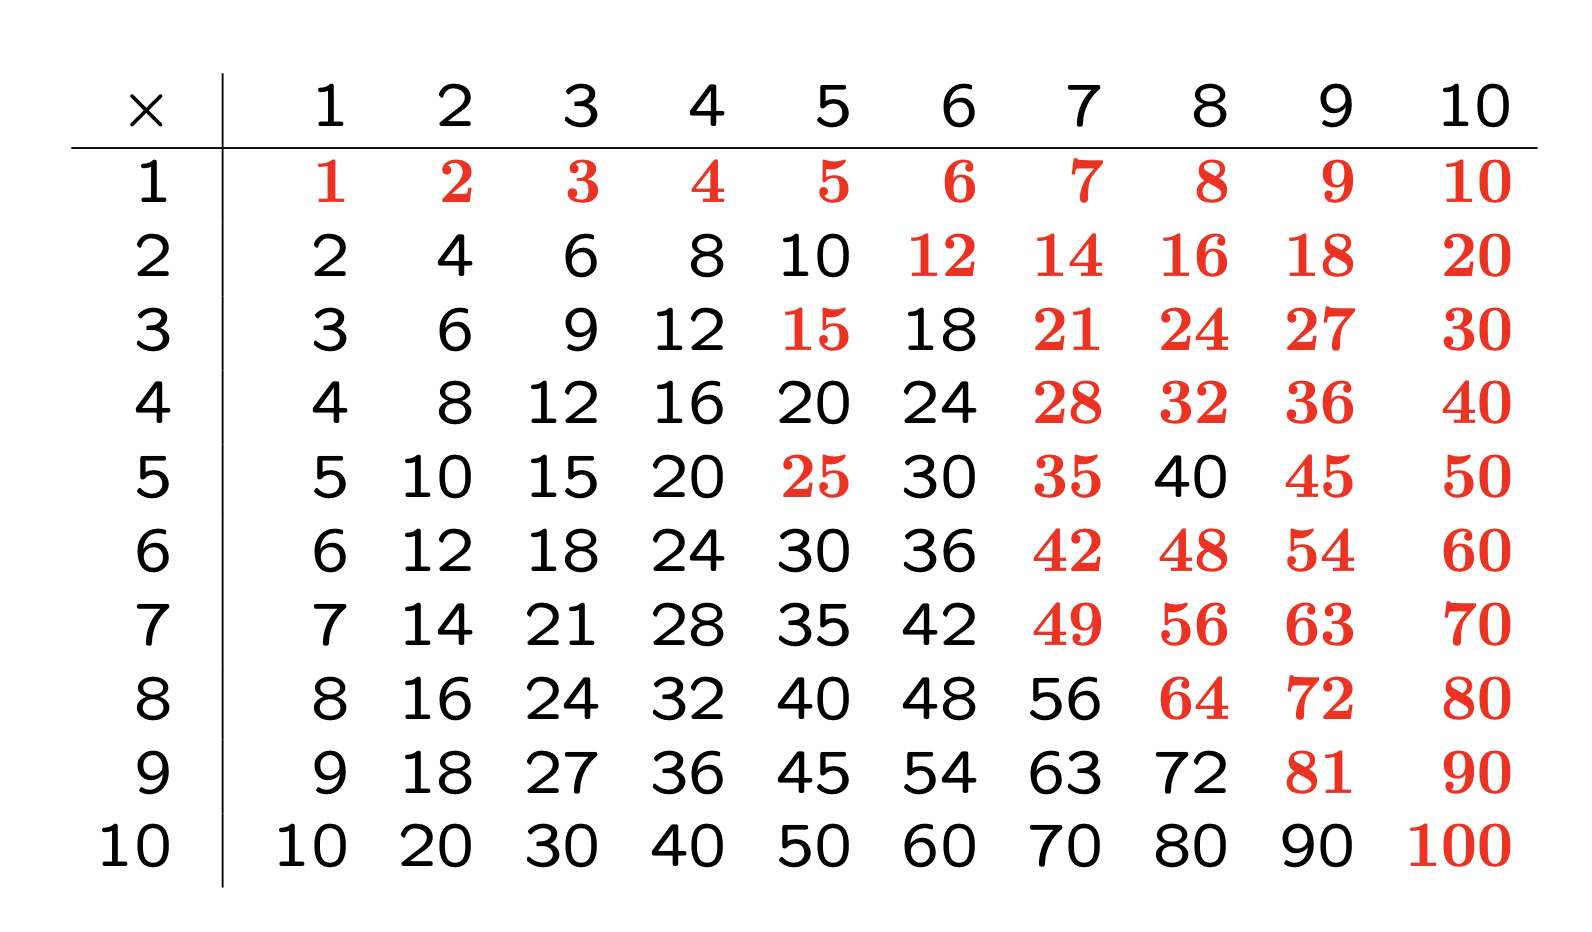
\includegraphics[width=0.6\textwidth]{mult-table.png}
    \caption{10 \(\times \) 10 multiplication table with distinct numbers highlighted in red.}
\end{figure}

These theorems are just bounds on the asymptotic behavior of \(\left\lvert [n] \cdot [n] \right\rvert \). 
In \cite{Ford}, Kevin Ford proved that the exact order of this quantity is
\[
    \left\lvert [n] \cdot [n] \right\rvert \asymp \frac{n^{2}}{\log \left( n^{2} \right) ^{\delta} \left( \log \log \left( n^{2} \right) \right) ^{\frac{3}{2} } } 
,\]
where
\[
    \delta = 1 - \frac{1 + \log \log \left( 2 \right)  }{2} 
.\]
The exact asymptotic behavior of this quantity is not known. 
To prove these, we require a lemma and a prerequisite theorem.

\begin{lemma*}
Let \(\left( a_{n}  \right) _{n = 1} ^{\infty }\) be a sequence of real numbers. Let \(A: \mathbb{R} \to \mathbb{R} \) be defined by
\[
    A(t) = \sum _{n \leq t} a_{n} 
.\]
For \(x \in \mathbb{R} \) and any differentiable function \(\phi : [1,y] \to \mathbb{R} \),
\[
    \sum _{n \leq x} a_{n} \phi(n) = A(x)\phi(x) - A(1) \phi(1) - \int_{1}^{x} A(t)\phi'(t) ~\mathrm{d} t
\]
\end{lemma*}

\textbf{FINISH THIS LATER}
\begin{proof}
\begin{align*}
    \sum _{x < n \leq y} a_{n} \phi(n) & = a_{\left\lceil x \right\rceil } \phi(\left\lceil x \right\rceil ) + \cdots  + a_{\left\lfloor y \right\rfloor } \phi(\left\lfloor y \right\rfloor )\\
    & = \left( A(x + 1) - A(x) \right) \phi(\left\lceil x \right\rceil ) + \cdots + \left( A(y) - A(y-1) \right) \phi(\left\lfloor y \right\rfloor ) \\
    & = \\
    & = A(y) \phi\left( \left\lfloor y \right\rfloor \right)  - A(x)\phi\left( \left\lceil x \right\rceil  \right) + \sum_{i= 1 }^{} \left( \phi\left( \left\lceil x \right\rceil + i \right) - \phi\left( \left\lceil x \right\rceil + 1 + i \right) \right) A(x + i)  
\end{align*}
\end{proof}

A prerequisite theorem gives the order of magnitude of 3 functions which
will prove useful.

\begin{theorem}
Define the functions \(\theta,\psi, \pi : [1, \infty) \to \mathbb{R} \) by
\[
    \theta(x) = \sum _{\substack{ p \leq x \\ p \text{ prime}  }} \log \left( p \right) 
,\]
\[
    \psi(x) = \sum _{\substack{ p^{\alpha} \leq x \\ p \text{ prime} \\ \alpha \in \mathbb{N}  }} \log \left( p \right) 
,\]
\[
    \pi(x) = \sum _{\substack{ p \leq x \\ p \text{ prime}  }} 1
.\]
We have
\[
    \psi(x) \asymp \theta(x) \asymp x
\]
and
\[
    \pi(x) \asymp \frac{x}{\log \left( x \right) } 
.\]
\end{theorem}

\begin{proof}
The functions \(\theta\) and \(\psi\) are clearly related by
\[
    \psi(t) = \prod _{\substack{ p \leq N^{\frac{1}{\alpha} } \\ p \text{ prime} \\ \alpha \in \mathbb{N}  }} \log \left( p \right) = \sum _{\alpha \in \mathbb{N} } \theta\left( t ^{\frac{1}{\alpha} } \right)  = \theta(t) + \sum _{\alpha \geq 2} \theta \left( t ^{\frac{1}{\alpha} } \right) 
.\]
Note that the sum over \(\alpha\) has only finitely many terms. The sum terminates when
\[
    2 \geq  t^{\frac{1}{\alpha} } \implies  \alpha \leq \log _{2} \left( t \right) 
.\]

A trivial upper bound on \(\theta (t)\) is
\[
    \theta(t) = \sum _{\substack{ p \leq t \\ p \text{ prime}}} \log \left( p \right) \leq t \log \left( t \right)  
,\]
so
\begin{align*}
    \psi(t) & = \theta(t) + \sum _{2 \leq \alpha \leq \log _{2} \left( t \right) } \theta(t ^{\frac{1}{\alpha} }) \\
    & \leq \theta(t) + \log _{2} \left( t \right) \theta(t^{\frac{1}{2} }) \\
    & \leq \theta(t) + \frac{t^{\frac{1}{2} }\log \left( t \right) ^{2}}{\log \left( 2 \right) }
\end{align*}
or
\[
    \psi(t) \ll \max \left( \theta(t), t^{\frac{1}{2} }\log \left( t \right) ^{2} \right) 
.\]
By showing \(\theta(t) \ll t\), we will have shown \(\psi(t) \ll \theta(t) \ll t\). Because \(\theta(t) \leq \psi(t)\),
we will have shown that \(\psi(t) \asymp \theta(t) \ll t\).

We have
\[
    \theta(t) = \sum _{\substack{ p \leq t \\ p \text{ prime}  }} \log \left( p \right) = \log \left( \prod _{\substack{ p \leq t \\  p \text{ prime}  }} p \right) 
,\]
so it is sufficient to show that
\[
    \prod _{\substack{ p \leq t \\ p \text{ prime}  }} p \ll e^{t}
.\]
It is also sufficient to prove it for \(t \in \mathbb{N} \) because \(\theta(t) = \theta\left( \left\lfloor t \right\rfloor  \right) \).

For some natural number \(t\), and a prime \(p\),
\[
    t + 1 < p \leq 2t + 1 \implies p \mid \binom{2t + 1}{t} = \frac{\left( 2t + 1 \right) !}{t! (t+1)!} 
.\]
Therefore, for any \(t\),
\[
    \prod _{\substack{ t + 1 < p \leq 2t + 1\\ p \text{ prime}   }} p   \mid \binom{2t+1}{t} \implies \prod _{\substack{ t + 1 < p \leq 2t + 1\\ p \text{ prime}   }} p   \leq  \binom{2t+1}{t}
,\]
which gives us
\[
    2 \prod _{\substack{ t + 1 < p \leq 2t + 1\\ p \text{ prime}   }} p   \leq  2 \binom{2t+1}{t} \leq (1+1)^{2t + 1} \implies \prod _{\substack{ t + 1 < p \leq 2t + 1\\ p \text{ prime}   }} p  \leq 4^{t}
.\]

The rest follows by induction on \(t\). Because we are proving
a statement about order of magnitude, the base case is trivial. Now suppose that
for some \(t \in \mathbb{N} \),
\[
    \prod _{\substack{ p \leq m \\p \text{ prime}  }} p \ll e^{t}
.\]
If \(t\) is odd, the induction follows trivially. If \(t\) is even, let \(t = 2m\),
so
\[
    \prod  _{\substack{ p \leq 2m \\ p \text{ prime}  }} p\ll e^{2m}
.\]
We have
\begin{align*}
\prod _{\substack{ p \leq 2m + 1 \\ p \text{ prime}  }} p & = \prod _{\substack{ p \leq m + 1 \\ p \text{ prime}  }} p \prod _{\substack{ m + 1 < p \leq 2m + 1 \\ p \text{ prime}  }} p \\
& \ll e^{m + 1} 4^{m} \\
& \ll e^{m+1} e^{m} = e^{2m+1}. 
\end{align*}
Thus, \(\psi(t) \asymp \theta(t) \ll t\). To prove \(\psi(t) \asymp \theta(t) \asymp t\),
it suffices to show that \(\psi(t) \gg t\).

\end{proof}

The final lemma needed is
\begin{lemma*}
\[
    \sum _{\substack{ p \leq n \\ p\text{ prime}  }} \frac{1}{p}  = \log\log \left( n \right) + O(1)
.\]
\end{lemma*}

\begin{proof}[Proof of Lemma]
Observe that for some number \(N \in \mathbb{N} \), the prime factorization of \(N!\) is of the form
\[
    N! = \prod _{\substack{ p \leq N \\ p \text{ prime}  }} p ^{\alpha(N,p)}
,\]
where
\[
    \alpha(N,p) = \sum _{i \in \mathbb{N} } \left\lfloor \frac{N}{p ^{i}}  \right\rfloor = \sum _{i \leq \log _{p} \left( N \right) } \left\lfloor \frac{N}{p ^{i}}  \right\rfloor  =\sum _{i \leq \log _{2} \left( N \right) } \left\lfloor \frac{N}{p ^{i}}  \right\rfloor 
.\]
It follows that
\begin{align*}
    \log \left( N! \right) & = \sum _{\substack{ p \leq N \\p \text{ prime}  }} \alpha(N,p) \log \left( p \right) \\
    & = \sum _{\substack{ p \leq N \\p \text{ prime} \\ i \leq \log _{p} \left( N \right)   }} \left\lfloor \frac{N}{p ^{i}}  \right\rfloor \log \left( p \right) \\
    & = \sum _{\substack{ p \leq N \\ p \text{ prime} \\ i \leq \log _{p} \left( N \right)  }} \left( \frac{N}{p ^{i}} - \delta(p) \right) \log \left( p \right) \\
    & = N\sum _{\substack{ p \leq N \\ p \text{ prime} \\ i \leq \log _{p} \left( N \right) }} \frac{\log \left( p \right) }{p ^{i}} - \sum _{\substack{ p \leq N \\ p \text{ prime} \\ i \leq \log _{p} \left( N \right)  }} \delta(p) \log \left( p \right) .
\end{align*}
We have that
\[
    i \leq \log _{p} \left( N \right) \iff p ^{i} \leq N
,\]
so
\[
    \sum  _{\substack{ p \leq N \\ p \text{ prime} \\ i \leq \log _{p} \left( N \right)  }} \log \left( p \right) = \psi(N)
,\]
and therefore
\[
    \sum _{\substack{ p \leq N \\ p \text{ prime} \\ i \leq \log _{2} \left( N \right)  }} \frac{\log \left( p \right) }{p ^{i}} \leq  \frac{\log \left( N! \right) }{N} + \frac{\psi(N)}{N} 
.\]

We also have, via a Riemann sum,
\begin{align*}
    \log \left( N! \right) & = \sum_{i=1}^{N} \log \left( i \right) \\
    & = \int_{2}^{N} \log \left( i \right)  ~\mathrm{d} i + O(1) \\
    & = \left. \left[ i\log \left( i \right) - i \right]  \right|_{i = 1}^{N} + O(1)\\
    & = N \log \left( N \right) - N + O(1).
\end{align*}

This leads to
\[
    \sum _{\substack{ p \leq N \\ p \text{ prime} \\ i \leq \log _{2} \left( N \right) }} \frac{\log \left( p \right) }{p ^{i}} = \frac{N \log \left( N \right) - N + O(1)}{N} + \frac{O(N)}{N} = \log \left( N \right)  + O(1)
.\]

Moreover, we have that
\begin{align*}
\sum  _{\substack{ p \leq N \\ p \text{ prime} \\ 2 \leq i \leq \log _{2} \left( N \right)  }} \frac{\log \left( p \right) }{p ^{i}} & \leq \sum  _{\substack{ x,i \geq 2}} \frac{\log \left( x \right) }{x ^{i}} \\
& = \sum _{x \geq 2} \sum _{i \geq 2} \frac{\log \left( x \right) }{x^{i}} \\
& = \sum _{x \geq 2} \frac{1}{x^{2}} \left( \frac{\log \left( x \right) }{1-\frac{1}{x} }  \right)\\
& = \sum _{x \geq 2} \frac{\log \left( x \right) }{x ^{2} - x} 
\end{align*}
which, by the limit comparison test, converges if
\[
    \sum _{x \geq 2} \frac{\log \left( x \right) }{x^{2}}
\]
converges.

Apply L'Hopital's rule to see that
\[
    \forall \epsilon > 0 ~,~ \log \left( x \right) = o(x^{\epsilon})
,\]
and therefore that
\begin{align*}
\sum _{x \geq 2} \frac{\log \left( x \right)}{x ^{2}} & = \sum _{x\geq 2} \frac{o(1)}{x^{2 - \epsilon}} \\
& \ll \sum _{x \geq 2} \frac{1}{x^{2-\epsilon}} \\
& \asymp \int_{2}^{\infty} \frac{1}{x^{2-\epsilon}}  ~\mathrm{d} x 
\end{align*}
which converges for \(\epsilon < 1\). It follows that
\[
    \sum _{\substack{ p \leq N \\p \text{ prime}  }}\frac{ \log \left( p \right) }{p} = \log \left( N \right) + O(1)
.\]

Applying Abel's summation formula,
\begin{align*}
\sum  _{\substack{ p \leq N \\p \text{ prime}  }} \frac{1}{p} & = \sum _{\substack{ p \leq N \\ p \text{ prime}  }}   \frac{\log \left( p \right) }{p} \cdot \frac{1}{\log \left( p \right) } \\
& = \left( \sum _{\substack{ p \leq N \\ p \text{ prime}  }} \frac{\log \left( p \right) }{p}  \right) \cdot \frac{1}{\log \left( N \right) } + O(1) + \int_{2}^{N} \frac{ \sum _{\substack{ p \leq t \\ p \text{ prime}  }}\frac{ \log \left( p \right) }{p} }{t \log ^{2}\left( t \right) }  ~\mathrm{d} t \\
& = \frac{ \log \left( N \right) + O(1)  }{\log \left( N \right) } + O(1) + \int_{2}^{N} \frac{\log \left( t \right) + O(1)}{t \log ^{2}\left( t \right) }  ~\mathrm{d} t\\
& = O(1) + \int_{2}^{N} \frac{1}{t \log \left( t \right) }  ~\mathrm{d} t + \int_{2}^{N} \frac{O(1)}{t \log ^{2}\left( t \right) }  ~\mathrm{d} t 
\end{align*}




\end{proof}

\end{document}